\documentclass[aspectratio=169]{beamer}

\mode<presentation>

\usepackage[utf8]{inputenc}
\usepackage[T1]{fontenc}	%makes å,ä,ö etc. proper symbols
\usepackage{amsmath}
\usepackage{graphicx}
\usepackage{xcolor}
\usepackage{listings}
\usepackage{multicol}
\usepackage{hyperref}
\usepackage[swedish]{babel}

\definecolor{LundaGroen}{RGB}{00,68,71}
\definecolor{StabilaLila}{RGB}{85,19,78}
\definecolor{VarmOrange}{RGB}{237,104,63}

\definecolor{MagnoliaRosa}{RGB}{251,214,209}
\definecolor{LundaHimmel}{RGB}{204,225,225}
\definecolor{LundaLjus}{RGB}{255,242,191}

\usefonttheme{serif}
\usetheme{malmoe}
\setbeamercolor{palette primary}{bg=LundaHimmel, fg=StabilaLila}
\setbeamercolor{palette quaternary}{bg=LundaGroen, fg=MagnoliaRosa}
\setbeamercolor{background canvas}{bg=LundaLjus}
\setbeamercolor{structure}{fg=LundaGroen}

\usepackage[many]{tcolorbox}

\newtcolorbox{cross}{blank,breakable,parbox=false,
  overlay={\draw[red,line width=5pt] (interior.south west)--(interior.north east);
    \draw[red,line width=5pt] (interior.north west)--(interior.south east);}}
    
\newcommand{\code}[1]{\colorbox{white}{\lstinline{#1}}}



\lstset{language=Python} 
\lstset{%language=[LaTeX]Tex,%C++,
    morekeywords={PassOptionsToPackage,selectlanguage,True,False},
    keywordstyle=\color{blue},%\bfseries,
    basicstyle=\small\ttfamily,
    %identifierstyle=\color{NavyBlue},
    commentstyle=\color{red}\ttfamily,
    stringstyle=\color{VarmOrange},
    numbers=left,%
    numberstyle=\scriptsize,%\tiny
    stepnumber=1,
    numbersep=8pt,
    showstringspaces=false,
    breaklines=true,
    %frameround=ftff,
    frame=single,
    belowcaptionskip=.75\baselineskip,
	tabsize=4,
	backgroundcolor=\color{white}
    %frame=L
}


\begin{document}

\lstset{literate=
  {á}{{\'a}}1 {é}{{\'e}}1 {í}{{\'i}}1 {ó}{{\'o}}1 {ú}{{\'u}}1
  {Á}{{\'A}}1 {É}{{\'E}}1 {Í}{{\'I}}1 {Ó}{{\'O}}1 {Ú}{{\'U}}1
  {à}{{\`a}}1 {è}{{\`e}}1 {ì}{{\`i}}1 {ò}{{\`o}}1 {ù}{{\`u}}1
  {À}{{\`A}}1 {È}{{\'E}}1 {Ì}{{\`I}}1 {Ò}{{\`O}}1 {Ù}{{\`U}}1
  {ä}{{\"a}}1 {ë}{{\"e}}1 {ï}{{\"i}}1 {ö}{{\"o}}1 {ü}{{\"u}}1
  {Ä}{{\"A}}1 {Ë}{{\"E}}1 {Ï}{{\"I}}1 {Ö}{{\"O}}1 {Ü}{{\"U}}1
  {â}{{\^a}}1 {ê}{{\^e}}1 {î}{{\^i}}1 {ô}{{\^o}}1 {û}{{\^u}}1
  {Â}{{\^A}}1 {Ê}{{\^E}}1 {Î}{{\^I}}1 {Ô}{{\^O}}1 {Û}{{\^U}}1
  {œ}{{\oe}}1 {Œ}{{\OE}}1 {æ}{{\ae}}1 {Æ}{{\AE}}1 {ß}{{\ss}}1
  {ű}{{\H{u}}}1 {Ű}{{\H{U}}}1 {ő}{{\H{o}}}1 {Ő}{{\H{O}}}1
  {ç}{{\c c}}1 {Ç}{{\c C}}1 {ø}{{\o}}1 {å}{{\r a}}1 {Å}{{\r A}}1
  {€}{{\euro}}1 {£}{{\pounds}}1 {«}{{\guillemotleft}}1
  {»}{{\guillemotright}}1 {ñ}{{\~n}}1 {Ñ}{{\~N}}1 {¿}{{?`}}1
}

\AtBeginSection[ ]
{
\begin{frame}{Innehåll}
	\begin{multicols}{2}
    	\tableofcontents[currentsection]
    \end{multicols}
\end{frame}
}

\title{Listor}
\date{ht 23}
\author{Programmering 1}

\maketitle

\section{Repetition}

\subsection{Skapa lista}

\begin{frame}[fragile]
	\frametitle{Repetition}
	\framesubtitle{Skapa lista}
	
	\begin{lstlisting}
min_lista = [5,3,0,8,1]
ny_lista = ["Knatte", "Fnatte", "Tjatte"]	
	\end{lstlisting}
	
\end{frame}

\subsection{Index}

\begin{frame}[fragile]
	\frametitle{Repetition}
	\framesubtitle{Index}
	
	\begin{lstlisting}
ny_lista = ["Knatte", "Fnatte", "Tjatte"]
print(ny_lista[0])
print(ny_lista[1])
print(ny_lista[2])
	\end{lstlisting}
	
	\pause
	
	\begin{lstlisting}
Knatte
Fnatte
Tjatte
	\end{lstlisting}
	
\end{frame}

\begin{frame}[fragile]
	\frametitle{Repetition}
	\framesubtitle{Index}
	
	\begin{lstlisting}
ny_lista = ["Knatte", "Fnatte", "Tjatte"]
print(ny_lista[-1])
print(ny_lista[-2])
print(ny_lista[-3])
	\end{lstlisting}
	
	\pause
	
	\begin{lstlisting}
Tjatte
Fnatte
Knatte
	\end{lstlisting}
	
\end{frame}

\subsection{Ändra ett element}

\begin{frame}[fragile]
	\frametitle{Repetition}
	\framesubtitle{Ändra ett element}
	
	\begin{lstlisting}
min_lista = [5,3,0,8,1]
min_lista[2] = 9
min_lista[3] = 'a'
print(min_lista)
	\end{lstlisting}
	
	\pause
	
	\begin{lstlisting}
[5,3,9,'a',1]
	\end{lstlisting}
	
\end{frame}

\subsection{Lägg till element}

\begin{frame}[fragile]
	\frametitle{Repetition}
	\framesubtitle{Lägg till element}
	
	\begin{lstlisting}
en_lista = ["Frodo", "Sam"]
en_lista.append("Merry")
en_lista.insert(1,"Pippin")
print(en_lista)
	\end{lstlisting}
	
	\pause
	
	\begin{lstlisting}
["Frodo", "Pippin", "Sam", "Merry"]
	\end{lstlisting}
	
\end{frame}

\subsection{Ta bort element}

\begin{frame}[fragile]
	\frametitle{Repetition}
	\framesubtitle{Ta bort element}
	
	\begin{lstlisting}
en_lista = ["Frodo", "Pippin", "Sam", "Merry"]
en_lista.pop(1)
en_lista.pop()
en_lista.remove("Sam")
print(en_lista)
	\end{lstlisting}
	
	\pause
	
	\begin{lstlisting}
["Frodo"]
	\end{lstlisting}
	
\end{frame}

\section{List slicing}

\subsection{[start:slut]}

\begin{frame}[fragile]
	\frametitle{List slicing}
	\framesubtitle{[start:slut]}
	
	\begin{lstlisting}
en_lista = ["Frodo", "Pippin", "Sam", "Merry"]
print(en_lista[1:3])
	\end{lstlisting}
	\begin{lstlisting}
["Pippin", "Sam"]
	\end{lstlisting}
	\pause
	\begin{lstlisting}
print(en_lista[1:])
	\end{lstlisting}
	\begin{lstlisting}
["Pippin", "Sam", "Merry"]
	\end{lstlisting}
	\pause
	\begin{lstlisting}
print(en_lista[:2])
	\end{lstlisting}
	\begin{lstlisting}
["Frodo", "Pippin"]
	\end{lstlisting}
	
	
\end{frame}

\subsection{[start:slut:steg]}

\begin{frame}[fragile]
	\frametitle{List slicing}
	\framesubtitle{[start:slut:steg]}
	
	\begin{lstlisting}
cool_lista = [0,1,2,3,4,5,6,7,8,9]
print(cool_lista[::2])
	\end{lstlisting}
	\begin{lstlisting}
[0,2,4,6,8]
	\end{lstlisting}
	
	\pause
	
	\begin{lstlisting}
print(cool_lista[::-1])
	\end{lstlisting}
	\begin{lstlisting}
[9,8,7,6,5,4,3,2,1,0]
	\end{lstlisting}
	
	\pause
	
	\begin{lstlisting}
print(cool_lista[1:6:3])
	\end{lstlisting}
	\begin{lstlisting}
[1,4]
	\end{lstlisting}
	

\end{frame}

\section{Sträng till lista}

\subsection{Tecken för tecken}

\begin{frame}[fragile]
	\frametitle{Strängar till listor}
	\framesubtitle{Konvertering}
	
	\begin{lstlisting}
min_text = "Upp till kamp"
min_lista = list(min_text)
print(min_lista)
	\end{lstlisting}
	\pause
	\begin{lstlisting}
['U','p','p',' ','t','i','l','l',' ','k','a','m','p']
	\end{lstlisting}
	
\end{frame}

\subsection{Ord}

\begin{frame}[fragile]
	\frametitle{Strängar till listor}
	\framesubtitle{Bryt upp i ord}
	
	\begin{lstlisting}
min_text = "Upp till kamp"
min_lista = min_text.split()
print(min_lista)
	\end{lstlisting}
	
	\pause
	
	\begin{lstlisting}
['Upp', 'till', 'kamp']
	\end{lstlisting}
	
	Med \code{.split(x)} kan man stycka upp strängen varje gång \code{x} dyker upp.
	
\end{frame}

\subsection{Listor till strängar}

\begin{frame}[fragile]
	\frametitle{Listor till strängar}
	
	\begin{lstlisting}
min_lista = ["U", "p", "p", " ", "n", "e", "r"]
min_text = "".join(min_lista)
print(min_text)
	\end{lstlisting}
	
	\pause
	
	\begin{lstlisting}
"Upp ner"
	\end{lstlisting}
	
\end{frame}



\section{Köer och Stackar}

\begin{frame}
	\frametitle{Köer och Stackar}
	
	I programmering är struktur viktigt, två grundläggande sätt att strukturera data är med
	
	\begin{itemize}
		\item en kö
		\item en stack.
	\end{itemize}
	
	
	
\end{frame}

\subsection{En kö}

\begin{frame}
	\frametitle{Kö}
	
	\begin{center}
		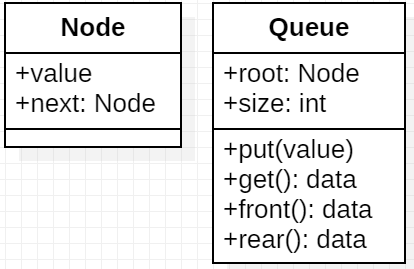
\includegraphics{kö.png}
	\end{center}
	
	En kö är en ordning där ''först in först ut gäller'' (FIFO, \textit{first in first out}) och fungerar som en kö i en affär. Då kan man lägga till element längst bak och plocka ut element längst fram
	
\end{frame}

\subsection{En stack}

\begin{frame}
	\frametitle{Stack}
	
	\begin{center}
		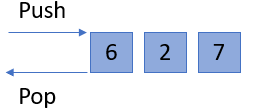
\includegraphics{stack.png}
	\end{center}
	
	En stack är en ordning där ''sist in först ut gäller'' (LIFO, \textit{last in first out}) och fungerar som en tallrikshög. Man lägger på nya tallrikar överst, och plockar alltid översta tallriken först.
	
	Vi kan enkelt simulera en stack i Python med listor om vi bara använder \code{.append(x)} och \code{.pop()}
	
\end{frame}


\section{Övningar}

\begin{frame}
	\frametitle{Övningar}
	
	\begin{itemize}
		\item Ladda ner filen \texttt{listor3.py}
	\end{itemize}

	\begin{enumerate}
		\item Dela upp \texttt{texten} i ord
		\item Hur många ord är det i texten?
		\item Räkna hur många ord som är exakt tre tecken långa.
		\item Dela nu istället upp texten i tecken. Hur många bokstäver finns det? Vilken bokstav är vanligast?
		\item Kryptera texten med ett Caesarchiffer.
	\end{enumerate}

\end{frame}



\end{document}